\begin{question}{24}{
    Bij de grenscontrole op Schiphol Airport onderzoekt de Koninklijke Marechaussee het verband tussen het aantal geopende controleloketten $X$ en de
    wachttijd $Y$ (in minuten) van reizigers naar een bestemming buiten het Schengengebied tijdens tien drukke ochtenden.
    {\par\bigskip
        \begin{center}
            \begin{tabular}{c|cccccccccc}
                \toprule
                    \textbf{$X$} & $2$ & $3$ & $4$ & $5$ & $6$ & $7$ & $8$ & $9$ & $10$ & $11$ \\
                \midrule
                    \textbf{$Y$} & $46.2$ & $41.3$ & $52.7$ & $36.1$ & $38.8$ & $41.6$ & $23.7$ & $11.0$ & $16.5$ & $14.2$ \\
                \bottomrule
            \end{tabular}
        \end{center}
    \par\bigskip}
}

    \subquestion{4}{
        Teken het spreidingsdiagram (scatter plot) op basis van de bovenstaande tabel.
        Geef hierbij ook duidelijk aan welke as welke variabele beschrijft.
    }
    \solution{
        De $x$-as duidt de onafhankelijke variabele $X$ uit, oftewel het aantal geopende controleloketten. \rubric{1}

        De $y$-as duidt de afhankelijke variabele $Y$ uit, oftewel de gemiddelde wachttijd van reizigers.\rubric{1}
        \begin{center}
            \resizebox{\textwidth}{!}{
                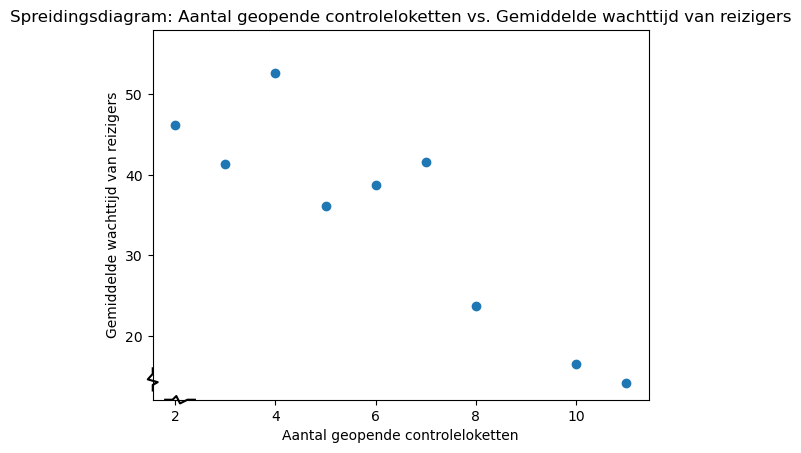
\includegraphics{exam20261106-scatterplot.png} \rubric{2}
            }
        \end{center}
    }

    \subquestion{7}{
        Bereken Pearson's correlatiecoëfficiënt $r(x,y)$ op basis van de data in de bovenstaande tabel.
        Wat zegt $r(x, y)$ over de relatie tussen het aantal geopende controleloketten en de wachttijd van reizigers?
    }
    \solution{
        We beginnen met het uitrekenen van Pearson's correlatiecoëfficiënt 
        \begin{align*}
            r(x, y)  &= \frac{ \overline{x \cdot y} - \overline{x} \cdot \overline{y} }{ \sqrt{ (\overline{x^2} - \overline{x}^2 ) \cdot (\overline{y^2} - \overline{y}^2) }}
        \end{align*}
        Hiervoor hebben we dus de waardes van $\overline{x}$, $\overline{y}$, $\overline{xy}$, $\overline{x^2}$ en $\overline{y^2}$ nodig.
        Deze bepalen we aan de hand van de volgende rekentabel:
        \begin{center}
            \begin{tabular}{ccccc}
                \toprule
                    $x$ & $y$ & $xy$ & $x^2$ & $y^2$ \\
                \midrule
    		        $2$  & $46.2$ & $92.4$  &   $4$ & $2134.44$ \\
                    $3$  & $41.3$ & $123.9$ &   $9$ & $1705.69$ \\
                    $4$  & $52.7$ & $210.8$ &  $16$ & $2777.29$ \\
                    $5$  & $36.1$ & $180.5$ &  $25$ & $1303.21$ \\
                    $6$  & $38.8$ & $232.8$ &  $36$ & $1505.44$ \\
                    $7$  & $41.6$ & $291.2$ &  $49$ & $1730.56$ \\
                    $8$  & $23.7$ & $189.6$ &  $64$ & $561.69$ \\
                    $9$  & $11.0$ & $99.0$  &  $81$ & $121.0$ \\
                    $10$ & $16.5$ & $165.0$ & $100$ & $272.25$ \\
                    $11$ & $14.2$ & $156.2$ & $121$ & $201.64$ \\
                \midrule
                    $\overline{x} = 6.5$ & $\overline{y} = 32.21$ & $\overline{xy} = 174.14$ & $\overline{x^2} = 50.5$ & $\overline{y^2} = 1231.321$ \rubric{3} \\ 
                \bottomrule
            \end{tabular}
        \end{center}
        \par\medskip
        De correlatiecoëfficiënt van Pearson is dus gelijk aan
        \begin{align*}
            r(x,y)  &= \frac{ \overline{x \cdot y} - \overline{x} \cdot \overline{y} }{ \sqrt{ (\overline{x^2} - \overline{x}^2) \cdot (\overline{y^2} - \overline{y}^2) } }\\
                    &= \frac{ 174.14 - 6.5 \cdot 32.21 }{ \sqrt{ (50.5 - 6.5^2) \cdot (1231.321 - 32.21^2) } } \\
                    &= \frac{-35.225}{39.9894} \\
                    &\approx -0.8809.
        \end{align*}
        De correlatiecoëfficiënt $r \approx -0.8809$ ligt ver van $0$ af en is negatief.
        Dit houdt in dat er een sterke negatieve lineaire (dalende) trend is. \rubric{1}
        Een groter aantal geopende controleloketten correleert sterk met een lagere wachttijd. \rubric{1}

        (Maximaal $2$ punten indien de student een positieve waarde heeft berekend voor $r(x, y)$ 
        en inziet dat dit niet rijmt met het spreidingsdiagram.
        $0$ punten indien de student dit besef niet laat zien in zijn/haar uitwerking.)
    }

    \subquestion{6}{
        Bereken de coëfficiënten $a$ en $b$ van de regressielijn $\hat{Y} = a + b \cdot X$.
        Bepaal aan de hand van de regressielijn een statistisch verantwoorde voorspelling voor de wachttijd van 
        reizigers op een willekeurige drukke dag wanneer er zes loketten geopend zijn.
    }
    \solution{
        Om de coëfficiënten $a$ en $b$ van de regressielijn te berekenen, gaan we de rekentabel van vraag (a) hergebruiken.
        Er volgt namelijk dat
        \begin{align*}
            b &= \frac{\overline{xy} - \overline{x} \cdot \overline{y}}{\overline{x^2} - (\overline{x})^2} \\
              &= \frac{174.1400 - 6.5 \cdot 32.21}{50.5 - (6.5)^2} \\
              &= \frac{-35.225}{8.25} \approx -4.2697 \\
            a &= \overline{y} - b \cdot \overline{x} \\
              &= 32.21 - -4.2697 \cdot 6.5 \\
              &\approx 59.9630.
        \end{align*}
        De formule van de regressielijn behorende bij deze steekproef is dus gelijk aan $Y = 59.9630-4.2697 \cdot X$. \rubric{1}
        Een statistisch verantwoorde voorspelling voor de wachttijd wanneer zes loketten zijn geopend
        vinden we door $x_0 = 6$ in te vullen:
        Dit geeft een waarde van $\hat{Y}_0 = 59.9630 - 4.2697 \cdot 6 \approx 34.3448$, oftewel 
        onze voorspelling zegt dat bij zes geopende loketten reizigers ruim $34$ minuten moeten wachten. \rubric{1} 

        (Geen punten indien $b > 0$ of extreem grote of kleine waarden voor $a$ en $b$ zonder besef dat dit niet kan kloppen. \\
        Maximaal $2$ punten indien de coëfficiënten dusdanige waarden hebben dat deze niet logischerwijs een passende lijn vormen door de steekproefdata.)
    }

    \subquestion{7}{
        Bereken een \SI{95}{\percent}-voorspellingsinterval voor de wachttijd van reizigers op een willekeurige dag waarop er zes loketten zijn geopend.
        Rond het interval af op gehele minuten zodat de betrouwbaarheid van het interval gewaarborgd blijft.
    }
    \solution{
        In opdracht (d) hebben we een puntschatting van $\hat{Y}_0 = 59.9630 - 4.2697 \cdot 6 \approx 34.3448$ bepaald.
        Daarnaast kunnen we de standaardafwijking $\sigma$ van de storingsterm $\varepsilon$ schatten:
        \begin{align*}
            s_{\varepsilon} &= \sqrt{ \frac{n}{n-2} \cdot \left( \overline{y^2} - a \cdot \overline{y} - b \cdot \overline{xy} \right) } \\ 
                               &= \sqrt{ \frac{10}{8} \cdot \left( 1231.321 - 59.9630 \cdot 32.21 - -4.2697 \cdot 174.14 \right) } \\ 
                               &\approx 7.3686.\rubric{2}
        \end{align*}

        Vervolgens kunnen we een puntschatting berekenen van de standaardafwijking van $Y$ voor gegeven $X = x_0$:
        \begin{align*}
            s_{f}   &= s_{\varepsilon} \cdot \sqrt{ 1 + \frac{1}{n} \cdot \left( 1 + \frac{(x_0 - \overline{x})^2}{\overline{x^2} - \overline{x}^2} \right) } \\
                    &= 7.3686 \cdot \sqrt{ 1 + \frac{1}{10} \cdot \left( 1 + \frac{(6 - 6.5)^2}{50.5 - 6.5^2} \right) } \\
                    &\approx 7.7389.\rubric{2}
        \end{align*}

        Omdat we de standaardafwijkingen geschat hebben en de storingstermen normaal verdeeld zijn, moeten we werken met de $t$-verdeling met $\df = n - 2 = 9$ vrijheidsgraden.
        De $t$-waarde die hoort bij een betrouwbaarheidsniveau $\alpha = 0.05$ is gelijk aan
        \[
            t = \invt(\opp = 1 - \alpha / 2, \df = n - 2) = \invt(\opp = 0.975, \df = 8) \approx 2.3060.\rubric{1}
        \]
        Het \SI{95}{\percent}-voorspellingsinterval voor $Y$ voor gegeven $X = 80$ kan dus worden beschreven door
        \begin{align*}
            &[\hat{Y}_0 - t \cdot s_{f}, \hat{Y}_0 - t \cdot s_{f}] \\
            &= [34.3448 - 2.3060 \cdot 7.7389; 34.3448 + 2.3060 \cdot 7.7389] \\ 
            &\approx [16.4990, 52.1907]. \rubric{1}
        \end{align*}
        
        Op een willekeurige drukke dag met zes geopende loketten moeten reizigers dus met \SI{95}{\percent} kans tussen
        $16$ en $53$ minuten wachten (dit is een heel groot interval, dus de nauwkeurigheid van de voorspelling is niet al te hoog;
        dit komt deels doordat de steekproefgrootte $n=10$ vrij klein is). \rubric{1}
    }
\end{question}